\documentclass[10pt]{article}
\usepackage[T1]{fontenc}

% Document Details
\newcommand{\CLASS}{AMATH 584}
\newcommand{\assigmentnum}{Assignment 8}

\usepackage[margin = 1.15in, top = 1.25in, bottom = 1.in]{geometry}

\usepackage{titling}
\setlength{\droptitle}{-6em}   % This is your set screw
\date{}
\renewcommand{\maketitle}{
	\clearpage
	\begingroup  
	\centering
	\LARGE \sffamily\textbf{\CLASS} \Large \assigmentnum\\[.8em]
	\large Tyler Chen\\[1em]
	\endgroup
	\thispagestyle{empty}
}
 % Title Styling
\usepackage{tocloft}
\renewcommand{\cfttoctitlefont}{\Large\sffamily\bfseries}
\renewcommand{\cftsecfont}{\normalfont\sffamily\bfseries}
\renewcommand{\cftsubsecfont}{\normalfont\sffamily}
\renewcommand{\cftsubsubsecfont}{\normalfont\sffamily}

\makeatletter
\let\oldl@section\l@section
\def\l@section#1#2{\oldl@section{#1}{\sffamily\bfseries#2}}

\let\oldl@subsection\l@subsection
\def\l@subsection#1#2{\oldl@subsection{#1}{\sffamily#2}}

\let\oldl@subsubsection\l@subsubsection
\def\l@subsubsection#1#2{\oldl@subsubsection{#1}{\sffamily#2}}
 % General Styling


\usepackage{enumitem}

% Figures
\usepackage{subcaption}

% TikZ and Graphics
\usepackage{tikz, pgfplots}
\pgfplotsset{compat=1.12}
\usetikzlibrary{patterns,arrows}
\usepgfplotslibrary{fillbetween}

\usepackage{pdfpages}
\usepackage{adjustbox}

\usepackage{lscape}
\usepackage{titling}
\usepackage[]{hyperref}


% Header Styling
\usepackage{fancyhdr}
\pagestyle{fancy}
\lhead{\sffamily \CLASS}
\rhead{\sffamily Chen \textbf{\thepage}}
\cfoot{}

% Paragraph Styling
\setlength{\columnsep}{1cm}
\setlength{\parindent}{0pt}
\setlength{\parskip}{5pt}
\renewcommand{\baselinestretch}{1}

% TOC Styling
\usepackage{tocloft}
\iffalse
\renewcommand{\cftsecleader}{\cftdotfill{\cftdotsep}}

\renewcommand\cftchapafterpnum{\vskip6pt}
\renewcommand\cftsecafterpnum{\vskip10pt}
\renewcommand\cftsubsecafterpnum{\vskip6pt}

% Adjust sectional unit title fonts in ToC
\renewcommand{\cftchapfont}{\sffamily}
\renewcommand{\cftsecfont}{\bfseries\sffamily}
\renewcommand{\cftsecnumwidth}{2em}
\renewcommand{\cftsubsecfont}{\sffamily}
\renewcommand{\cfttoctitlefont}{\hfill\bfseries\sffamily\MakeUppercase}
\renewcommand{\cftaftertoctitle}{\hfill}

\renewcommand{\cftchappagefont}{\sffamily}
\renewcommand{\cftsecpagefont}{\bfseries\sffamily}
\renewcommand{\cftsubsecpagefont}{\sffamily}
\fi
 % General Styling
% Code Display Setup
\usepackage{listings,lstautogobble}
\usepackage{lipsum}
\usepackage{courier}
\usepackage{catchfilebetweentags}

\lstset{
	basicstyle=\small\ttfamily,
	breaklines=true, 
	frame = single,
	rangeprefix=,
	rangesuffix=,
	includerangemarker=false,
	autogobble = true
}


\usepackage{algorithmicx}
\usepackage{algpseudocode}

\newcommand{\To}{\textbf{to}~}
\newcommand{\DownTo}{\textbf{downto}~}
\renewcommand{\algorithmicdo}{\hspace{-.2em}\textbf{:}}
 % Code Display Setup
% AMS MATH Styling
\usepackage{amsmath, amssymb}
\newcommand{\qed}{\hfill\(\square\)}

%\newtheorem*{lemma}{Lemma} 
%\newtheorem*{theorem}{Theorem}
%\newtheorem*{definition}{Definition}
%\newtheorem*{prop}{Proposition}
%\renewenvironment{proof}{{\bfseries Proof.}}{}


% mathcal
\newcommand{\cA}{\ensuremath{\mathcal{A}}}
\newcommand{\cB}{\ensuremath{\mathcal{B}}}
\newcommand{\cC}{\ensuremath{\mathcal{C}}}
\newcommand{\cD}{\ensuremath{\mathcal{D}}}
\newcommand{\cE}{\ensuremath{\mathcal{E}}}
\newcommand{\cF}{\ensuremath{\mathcal{F}}}
\newcommand{\cG}{\ensuremath{\mathcal{G}}}
\newcommand{\cH}{\ensuremath{\mathcal{H}}}
\newcommand{\cI}{\ensuremath{\mathcal{I}}}
\newcommand{\cJ}{\ensuremath{\mathcal{J}}}
\newcommand{\cK}{\ensuremath{\mathcal{K}}}
\newcommand{\cL}{\ensuremath{\mathcal{L}}}
\newcommand{\cM}{\ensuremath{\mathcal{M}}}
\newcommand{\cN}{\ensuremath{\mathcal{N}}}
\newcommand{\cO}{\ensuremath{\mathcal{O}}}
\newcommand{\cP}{\ensuremath{\mathcal{P}}}
\newcommand{\cQ}{\ensuremath{\mathcal{Q}}}
\newcommand{\cR}{\ensuremath{\mathcal{R}}}
\newcommand{\cS}{\ensuremath{\mathcal{S}}}
\newcommand{\cT}{\ensuremath{\mathcal{T}}}
\newcommand{\cU}{\ensuremath{\mathcal{U}}}
\newcommand{\cV}{\ensuremath{\mathcal{V}}}
\newcommand{\cW}{\ensuremath{\mathcal{W}}}
\newcommand{\cX}{\ensuremath{\mathcal{X}}}
\newcommand{\cY}{\ensuremath{\mathcal{Y}}}
\newcommand{\cZ}{\ensuremath{\mathcal{Z}}}

% mathbb
\usepackage{bbm}
\newcommand{\bOne}{\ensuremath{\mathbbm{1}}}

\newcommand{\bA}{\ensuremath{\mathbb{A}}}
\newcommand{\bB}{\ensuremath{\mathbb{B}}}
\newcommand{\bC}{\ensuremath{\mathbb{C}}}
\newcommand{\bD}{\ensuremath{\mathbb{D}}}
\newcommand{\bE}{\ensuremath{\mathbb{E}}}
\newcommand{\bF}{\ensuremath{\mathbb{F}}}
\newcommand{\bG}{\ensuremath{\mathbb{G}}}
\newcommand{\bH}{\ensuremath{\mathbb{H}}}
\newcommand{\bI}{\ensuremath{\mathbb{I}}}
\newcommand{\bJ}{\ensuremath{\mathbb{J}}}
\newcommand{\bK}{\ensuremath{\mathbb{K}}}
\newcommand{\bL}{\ensuremath{\mathbb{L}}}
\newcommand{\bM}{\ensuremath{\mathbb{M}}}
\newcommand{\bN}{\ensuremath{\mathbb{N}}}
\newcommand{\bO}{\ensuremath{\mathbb{O}}}
\newcommand{\bP}{\ensuremath{\mathbb{P}}}
\newcommand{\bQ}{\ensuremath{\mathbb{Q}}}
\newcommand{\bR}{\ensuremath{\mathbb{R}}}
\newcommand{\bS}{\ensuremath{\mathbb{S}}}
\newcommand{\bT}{\ensuremath{\mathbb{T}}}
\newcommand{\bU}{\ensuremath{\mathbb{U}}}
\newcommand{\bV}{\ensuremath{\mathbb{V}}}
\newcommand{\bW}{\ensuremath{\mathbb{W}}}
\newcommand{\bX}{\ensuremath{\mathbb{X}}}
\newcommand{\bY}{\ensuremath{\mathbb{Y}}}
\newcommand{\bZ}{\ensuremath{\mathbb{Z}}}

% alternative mathbb
\newcommand{\NN}{\ensuremath{\mathbb{N}}}
\newcommand{\RR}{\ensuremath{\mathbb{R}}}
\newcommand{\CC}{\ensuremath{\mathbb{C}}}
\newcommand{\ZZ}{\ensuremath{\mathbb{Z}}}
\newcommand{\EE}{\ensuremath{\mathbb{E}}}
\newcommand{\PP}{\ensuremath{\mathbb{P}}}
\newcommand{\VV}{\ensuremath{\mathbb{V}}}
\newcommand{\cov}{\ensuremath{\text{Co}\VV}}
% Math Commands

\newcommand{\st}{~\big|~}
\newcommand{\stt}{\text{ st. }}
\newcommand{\ift}{\text{ if }}
\newcommand{\thent}{\text{ then }}
\newcommand{\owt}{\text{ otherwise }}

\newcommand{\norm}[1]{\left\lVert#1\right\rVert}
\newcommand{\snorm}[1]{\lVert#1\rVert}
\newcommand{\ip}[1]{\ensuremath{\left\langle #1 \right\rangle}}
\newcommand{\pp}[3][]{\frac{\partial^{#1}#2}{\partial #3^{#1}}}
\newcommand{\dd}[3][]{\frac{\d^{#1}#2}{\d #3^{#1}}}
\renewcommand{\d}{\ensuremath{\mathrm{d}}}

\newcommand{\indep}{\rotatebox[origin=c]{90}{$\models$}}




 % Math shortcuts
% Problem
\usepackage{floatrow}

\newenvironment{problem}[1][]
{\pagebreak
\noindent\rule{\textwidth}{1pt}\vspace{0.25em}
{\sffamily \textbf{#1}}
\par
}
{\par\vspace{-0.5em}\noindent\rule{\textwidth}{1pt}}

\newenvironment{solution}[1][]
{{\sffamily \textbf{#1}}
\par
}
{}

 % Problem Environment

\newcommand{\note}[1]{\textcolor{red}{\textbf{Note:} #1}}

\hypersetup{
   colorlinks=true,       % false: boxed links; true: colored links
   linkcolor=violet,          % color of internal links (change box color with linkbordercolor)
   citecolor=green,        % color of links to bibliography
   filecolor=magenta,      % color of file links
   urlcolor=cyan           % color of external links
}


\begin{document}
\maketitle

\begin{problem}[Exercise 26.1]
Theorem 26.1 and its successors in later lectures show that we can compute eigenvalues \( \{ \tilde{\lambda_k}\} \) of \( A \) numerically that are the exact eigenvalues of a matrix \( A+\delta A \) with \( \norm{\delta A}/\norm{A} = \mathcal{O}(\epsilon_{\text{mach}}) \). Does this mean they are close to the exact eigenvalues \( \{ \lambda_k \} \) of \( A \)? This is a question of eigenvalue perturbation theory.

    One can approach such problems geometrically as follows. Given \( A\in\CC^{m\times m} \) with spectrum \( \Lambda(A) \subseteq \CC \) and \( \epsilon > 0 \), define the 2-norm \( \epsilon \)-pseudospectrum of \( A \),  \( \Lambda_{\epsilon}(A) \), to be the set of numbers \( z\in\CC \) satisfying any of the following conditions:
    \begin{enumerate}[nolistsep]
        \item[(i)] \( z \) is an eigenvalue of \( A+\delta A \) for some \( \delta A \) with \( \norm{\delta A}_2\leq \epsilon \);
        \item[(ii)] There exists a vector \( u\in\CC^{m} \) with \( \norm{(A-zI)u}_2 \leq \epsilon \) and \( \norm{u}_2=1 \);
        \item[(iii)] \( \sigma_m(zI-A) \leq \epsilon \);
        \item[(iv)] \( \norm{(zI-A)^{-1}}_2 \geq \epsilon^{-1} \)
    \end{enumerate}
    
    The matrix \( (zI-A)^{-1} \) is known as the resolvent of \( A \) at \( z \). If \( z \) is an eigenvalue of \( A \), we use the convention \( \norm{(zI-A)^{-1}}_2 = \infty \). \( \sigma_m \) denotes the smallest singular value.

    Prove the above conditions are equivalent.

    Use the results of this exercise to show that if \(A\) is a normal matrix and \(\tilde{\lambda}\) is an eigenvalue of \(A+ \delta A\) for some \(\delta A\) with \(\| \delta A \|_2 \leq \epsilon\), then there is an eigenvalue \(\lambda\) of \(A\) such that \(| \tilde{\lambda} - \lambda | \leq \epsilon\).  Would you say that the problem of computing eigenvalues of a normal matrix is well-conditioned or ill-conditioned?
\end{problem}

\begin{solution}[Solution]
(i) \( \Rightarrow \) (ii) Suppose \( z \) is an eigenvalue of \( A+\delta A \) for some \( \delta A \) with \( \norm{\delta A} \leq \epsilon \). Let \( u \) be a corresponding eigenvector with \( \norm{u}=1 \). Then, \( (A+\delta a) u = z u \) so \( Au-zu = (A-zI)u = -\delta Au \). Taking the norm of each side we have, \( \norm{(A-zI)u}_2 = \norm{-\delta A u} \leq \norm{\delta A}\norm{u} \leq \epsilon \).

(ii) \( \Rightarrow \) (iii) The smallest singular value, \( \sigma_m \) is minimum stretch of a vector under \( (zI-A) \). That is, \( \norm{(zI-A)v} \geq \sigma_m \norm{v} \) for all \( v \). Therefore, in particular, \( \sigma_m(zI-A) \leq \norm{(zI-A)u}/{\norm{u}} = \norm{(zI-A)u} \leq \epsilon \).

(iii) \( \Rightarrow \) (iv) Recall the largest singular value of a matrix is the reciprocal of the smallest singular value of its inverse. We then have, \( \norm{(zI-A)^{-1}}_2 = \sigma_{\text{max}}((zI-A)^{-1})= \sigma_{\text{min}}(zI-A)^{-1}\geq \epsilon^{-1} \)

(iv) \( \Rightarrow \) (i) Let \( u,v \) be the first left and right singular vectors of \( (zI-A)^{-1} \) with singular value \( \sigma^{-1} := \norm{(zI-A)^{-1}} \). Then \( \norm{u} = \norm{v} = 1 \) and \( \sigma \leq \epsilon \) and by definition, \( (zI-A)^{-1}v = \sigma^{-1} u \). Rearranging we have, \( \sigma v = (zI-A) u \) so \( (A-\sigma vu^*)u = Au-\sigma v u^*u = Au-\sigma v = zu \). This means \( z \) is an eigenvector of \( A-\sigma v u^* \) and \( \norm{\sigma v u^*} = \sigma \norm{v} \norm{u^*} = \sigma \leq \epsilon \).

This proves the four statements are equivalent. \qed

Suppose \( A \) is a normal matrix and \( \tilde{\lambda} \) is an eigenvalue of \( (A+\delta A) \) for some \( \delta A \) with \( \norm{\delta A} \leq \epsilon \).

Since \( A \) is normal, it has a unitary diagonalization, \( A=U\Lambda U^* \). Then \( A-zI = U\Lambda U^* - z UIU^* = U(\Lambda-zI)U^* \). We can write this as an SVD by moving the any negative entries of \( \Lambda-zI \) to the \( U \) on the left. We write the SVD as, \( A = U|\Lambda-zI|U^* \), noting that \( U \) might have different signs than before.

By hypothesis, \( \tilde{\lambda} \) is an eigenvalue of \( A+\delta A \) where \( \norm{\delta A}\leq \epsilon \). Equivalently, \( \sigma_m:=\sigma_m(\tilde{\lambda}I-A) \leq \epsilon \). From the SVD above we have, \( \sigma_m u =  (\tilde{\lambda}I-A)u = U|zI-\Lambda|U^*u \), where \( u \) is the last singular vector (the one corresponding to \( \sigma_m \)). So \( \sigma_m U^*u = | \tilde{\lambda}I-\Lambda|U^*u \). Then looking at bottom entry of these vectors we have \( | \tilde{\lambda} -\lambda_m| = \sigma_m \leq \epsilon \).

Since \( \lambda_m \) is an entry of \( \Lambda \), \( \lambda_m \) is an eigenvalue of \( A \). The result is then proved. \qed

The problem of computing eigenvalues of a normal matrix is well conditioned since a small change in \( A \) leads to a similarly small change in the eigenvalues. 

\end{solution}

\begin{problem}[Exercise 2]
Let
\begin{align*}
    A = \left[ \begin{array}{ccc} 0 & 1 & 0 \\ 0 & 0 & 1 \\ 0 & 0 & 0 \end{array} \right] &&
A_{\epsilon} = \left[ \begin{array}{ccc} 0 & 1 & 0 \\ 0 & 0 & 1 \\ \epsilon & 0 & 0 \end{array} \right] .
\end{align*}
What are the eigenvalues of \(A\) and of \(A_{\epsilon}\)?  Would you say that the problem of computing the eigenvalues of a matrix \(A\) of this form is well-conditioned or ill-conditioned?  
\end{problem}

\begin{solution}[Solution]
We have,
\begin{align*}
    p_A(z) &= \det(A-zI) = -z \det \left[\begin{array}{cc}-z & 1 \\ 0 & -z\end{array}\right] = -z^3 \\ 
        p_{A_{\epsilon}}(z) &= \det(A_{\epsilon}-zI) 
        = -z \det \left[\begin{array}{cc}-z & 1 \\ 0 & -z\end{array}\right] 
            + \epsilon \det \left[\begin{array}{cc}1&0\\0&1\end{array}\right]
        = -z^3 + \epsilon
\end{align*}

Therefore the eigenvalues of \( A \) are all zero, and the eigenvalues of \( A_{\epsilon} \) are \( \epsilon^{1/3}, \epsilon^{1/3}e^{2\pi i/3}, \epsilon^{1/3}e^{4 \pi i /3}  \).


We consider the problem of computing eigenvalues as a map \( f:\CC^{m\times m} \to \CC^m \), where the input is a matrix, and the output is a vector of the eigenvalues.

The relative condition number is not a very useful measure of the conditioning of a problem when the input or output to the unperturbed problem is zero.

The absolute condition number is,
\begin{align*}
    \kappa := \lim_{\delta \to 0} \sup_{\norm{\delta x}\leq \delta } \left( \dfrac{\norm{\delta f}}{\norm{\delta x}} \right)
\end{align*}

In this case, we have \( \norm{\delta A} = \norm{A-A_\epsilon} = \epsilon \) and \( \norm{A} = 1 \). Likewise, we have \( \norm{f(A)} = \norm{[0,0,0]} = 0 \) and \( \norm{f(\delta A)} = \norm{[ \epsilon^{1/3}, \epsilon^{1/3}e^{2\pi i/3}, \epsilon^{1/3}e^{4 \pi i /3}  ]} = 3^{1/3} \epsilon^{1/3} \). Therefore,
\begin{align*}
    \kappa \geq \left( \dfrac{\norm{\delta f}}{\norm{\delta x}} \right) 
    =\left( \dfrac{3^{1/3}\epsilon^{1/3}}{\epsilon} \right) \geq \epsilon^{-2/3}
\end{align*}


If epsilon is small then this is large. That is, a small change to the problem leads to a large change to the output of the problem. Therefore, the problem of computing eigenvalues this matrix is ill conditioned. 

More generally, a matrix with zeros everywhere except for ones on the main superdiagonal will will have eigenvalues 0, and eigenvalues equal to the \( m \)-th roots of \( \epsilon \) when perturbed with an error of \( \epsilon \) in the bottom left corner. So, similar to this computation, calculating the eigenvalues of these matrices will never be well conditioned.

\end{solution}

\begin{problem}[Exercise 28.1]
What happens if you apply the unshifted QR algorithm to an orthogonal matrix? Figure out the answer, and then explain how it relates to Theorem 28.4.
\end{problem}

\begin{solution}[Solution]
The unshifted QR algorithm is,
\begin{lstlisting}[mathescape=true]
$A^{(0)} = A$
for $ k=1,2,... $:
    $[Q^{(k)}$,$R^{(k)}]$ = qr($A^{(k-1)}$)
    $A^{(k)} = R^{(k)}Q^{(k)}$
\end{lstlisting}

Suppose \( A \) is orthogonal. Then in the first step we have, \( [Q^{(1)},R^{(1)}] = [Q,I] \) since the QR decomposition of an orthogonal matrix is just itself times the identity. Then at each stage \( A^{(k)} = A^{(k-1)} \) so the algorithm will never converge.

If \( Q \) is orthogonal then all eigenvalues have magnitude 1. So the theorem is not satisfied since there is not distinct eigenvalue with largest magnitude.
\end{solution}

\begin{problem}[Exercise 4]
Consider the matrix
\begin{align*}
    A = \left[ \begin{array}{cccc} 2 & -1 & & \\ -1 & \ddots & \ddots & \\
 & \ddots & \ddots & -1 \\ & & -1 & 2 \end{array} \right] .
\end{align*}

    Taking \(A\) to be a \(10\) by \(10\) matrix, try the following:
\begin{enumerate}
    \item[(a)] What information does Gerschgorin's theorem give you about this matrix?
    \item[(b)] Implement the power method to compute an approximation to the eigenvalue of largest absolute value and its corresponding eigenvector.  [Note:  Use a random initial vector.  If you choose something special, like the vector of all \(1\)'s, it may turn out to be orthogonal to the eigenvector you are looking for.] Turn in a listing of your code together with the eigenvalue/eigenvector pair that you computed.  Once you have a good approximate eigenvalue, look at the error in previous approximations and comment on the rate of convergence of the power method.
    \item[(c)] Implement the QR algorithm (without shifts) to take \(A\) to diagonal form. You may use Matlab routine \verb+[Q,R] = qr(A);+ to perform the necessary QR decompositions.  Comment on the rate at which the off-diagonal entries in \(A\) are reduced.
    \item[(d)] Take one of the eigenvalues computed in your QR algorithm and, using it as a shift in inverse iteration, compute the corresponding eigenvector.
\end{enumerate}

\end{problem}

\begin{solution}[Solution]
Define,
\begin{lstlisting}
A = np.triu(np.tril(-np.ones((10,10))+3*np.identity(10),1),-1)
\end{lstlisting}

\begin{enumerate}
    \item[(a)] We know all the eigenvalues are found in the disk: \( \{z : |z-2| \leq 2 \} \). Since \( A \) is symmetric, (and therefore Hermetian) all eigenvalues are real. Therefore they all like within the closed interval \( [0,4] \).
    \item[(b)]
        We iterate until the Raleigh quotient changes by less than the specified tolerance (machine epsilon). The code is implemented in python as,
        \begin{lstlisting}
def power(A):
    tol=10e-16
    l=[0,1]
    v = np.random.rand(10)
    v = v/np.linalg.norm(v)
    while abs(l[-1] - l[-2]) > tol:
        w = A@v
        v = w/np.linalg.norm(w)
        l.append(v.T@A@v)
    return [l[-1],v]
        \end{lstlisting}
        This gives output,
        \begin{lstlisting}
[3.9189859472289839,
 array([ 0.1201312144953602, -0.2305301009433062,  0.3222527902846078,
        -0.3878684540194245,  0.4220613062809278, -0.4220612556116857,
         0.3878683180988246, -0.32225261226648  ,  0.2305299373471484,
        -0.1201311172617966])]
        \end{lstlisting}

        Figure~\ref{powercg} shows a  plot of the log of \( |\lambda^{(k)} - \lambda_\infty| \). As expected convergence is linear.
        \begin{figure}[H]\centering
            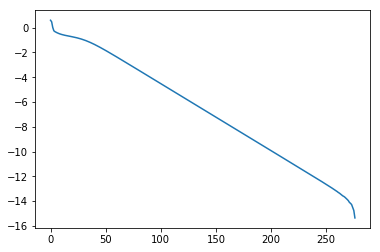
\includegraphics[width=.5\textwidth]{img/powercg.png}
            \caption{\(\log|\lambda^{k+1} - \lambda_\infty|\) }
            \label{powercg}
        \end{figure}
        
    
    \item[(c)]
        We implement the unshifted QR algorithm in python as,
\begin{lstlisting}
    def qr(A):
    tol=10e-16
    A_old = np.identity(len(A))
    while abs(A[0,0] - A_old[0,0]) > tol:
        [Q,R] = np.linalg.qr(A)
        A=R@Q
    
    return A
\end{lstlisting}

        Figure~\ref{qrod} shows a  plot of the log of the two norm of the entries of the first subdiagonal. It appears the convergence is linear
        \begin{figure}[H]\centering
            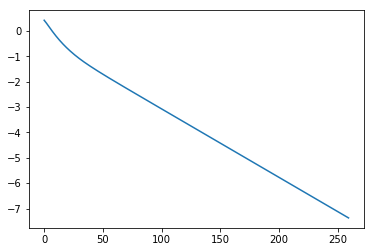
\includegraphics[width=.5\textwidth]{img/qrod.png}
            \caption{\(\log \norm{\left[A^{(k)}_{i,i+1}\right]_{i=1}^{m-1}}  \) vs iteration}
            \label{qrod}
        \end{figure}

    \item[(d)] 
        We implement inverse iteration in python as,
        \begin{lstlisting}
def inviter(A,s):
    tol=10e-16
    l=[0,1]
    v = np.random.rand(10)
    v = v/np.linalg.norm(v)
    while abs(l[-1] - l[-2]) > tol:
        w = np.linalg.solve(A-s*np.identity(len(A)),v)
        v = w/np.linalg.norm(w)
        l.append(v.T@A@v)

    return [l[-1],v]
        \end{lstlisting}

        Using {\tt s = qr(A)[3] = 2.8308300260037638 } we have output,
        \begin{lstlisting}
array([ 3.9189859472289963,  3.6825070656623637,  3.309721467890574 ,
        2.8308300260037744,  2.2846296765465772,  1.7153703234534301,
        0.0810140527710047,  0.3174929343376377,  0.6902785321094301,
        1.1691699739962271])
        \end{lstlisting}

\end{enumerate}
\end{solution}



\end{document}
